\chapter{Контрмера против атаки с навязыванием ключа} \label{ch:ch3}

%%%%%%%%%%%%%%%%%%%%%%%%%%%%%%%%%%%%%%%%%%%%%%%%%%%%%%%%%%%%%%%%%%%%%%%%%%%%%%%%%%%%%%%%%%%%%%%%%%%%%%%%%%%%%%%%%

\section{Атака с навязыванием ключа «поддельными» состояниями в системе квантовой коммуникации на боковых частотах} \label{sec:ch3/sec1}

 \begin{figure}[ht]
  \centering
  \includegraphics[scale=0.35]{images/scw-setup_FSA_rus1.pdf}
  \caption{Принципиальная оптическая схема предлагаемой атаки с <<поддельными состояниями>>}
  \label{fig:SCW_FSA}
\end{figure}

\pagebreak
%%%%%%%%%%%%%%%%%%%%%%%%%%%%%%%%%%%%%%%%%%%%%%%%%%%%%%%%%%%%%%%%%%%%%%%%%%%%%%%%%%%%%%%%%%%%%%%%%%%%%%%%%%%%%%%%%
\section{Границы применимости атаки с навязыванием ключа} \label{sec:ch3/sec2}

 \begin{figure}[ht]
  \centering
  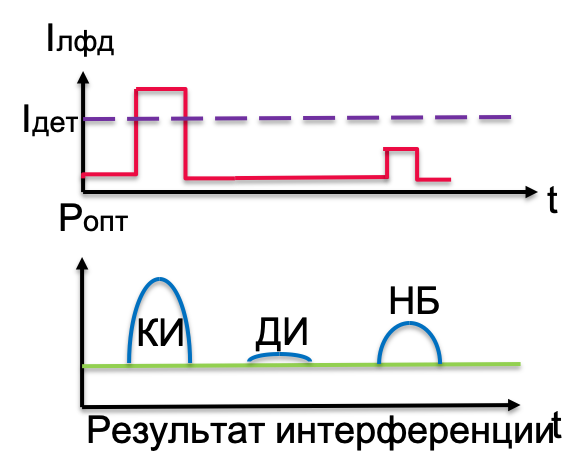
\includegraphics{Palways.png}
  \caption{Методика определения границ применимости}
  \label{fig:Palways}
\end{figure}


 \begin{figure}[ht]
  \centering
  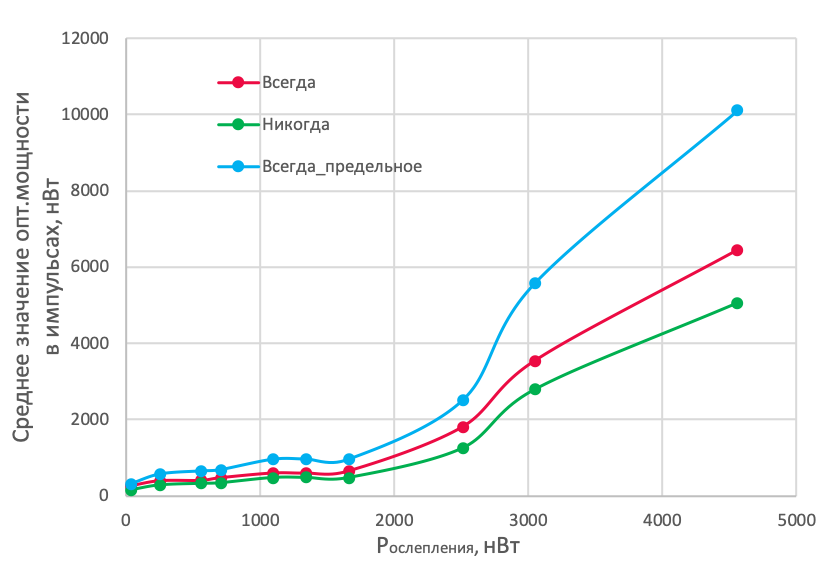
\includegraphics{Bounds.png}
  \caption{Границы применимости используемых оптических мощностей контролирующего импульса и засветки детектора}
  \label{fig:Bounds}
\end{figure}

\pagebreak
%%%%%%%%%%%%%%%%%%%%%%%%%%%%%%%%%%%%%%%%%%%%%%%%%%%%%%%%%%%%%%%%%%%%%%%%%%%%%%%%%%%%%%%%%%%%%%%%%%%%%%%%%%%%%%%%%
\section{Оценка возможностей злоумышленника при атаке с выведением детектора из режима Гейгера для систем квантовой коммуникации на боковых частотах} \label{sec:ch3/sec3}
 \begin{figure}[ht]
  \centering
  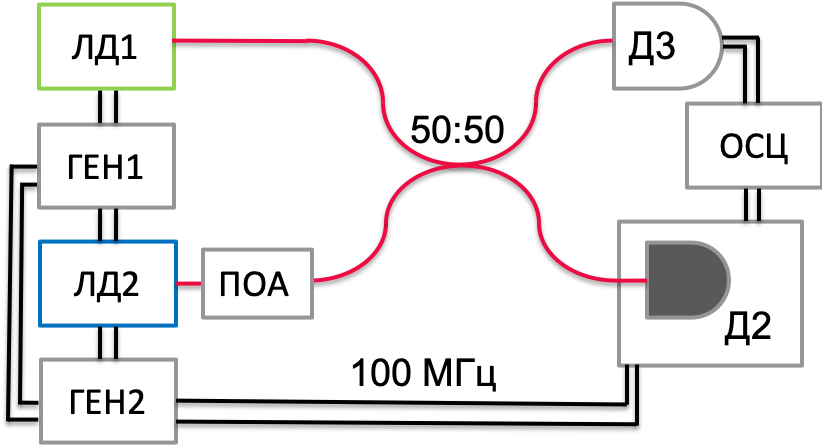
\includegraphics{Scheme_2.7.eps}
  \caption{Принципиальная оптическая схема эксперимента}
  \label{fig:Scheme_2.7}
\end{figure}

\begin{table}
	\caption{\label{tab:blinding}Calculated parameters for successful control of ID210 detector in SCW QKD scheme.}
	\begin{tabular}[t]{c c c c}
	\hline\hline
	\makecell{Eve's faked-state\\ power in...} & \makecell{Blinding\\ power ($\nano\watt$)} & $E_\text{always}$ ($\femto\joule$) & $E_\text{never}$ ($\femto\joule$) \\
	\hline
	\makecell{subcarriers after\\ filtering} & 35 & 25.8 & 15.4 \\
	\makecell{spectrum before\\ modulation} & 700 & 516 & 308 \\
	\makecell{spectrum entering\\ Bob's module} & 3056 & 2252 & 1345 \\
	\hline\hline
	\end{tabular}
\end{table}


\pagebreak
%%%%%%%%%%%%%%%%%%%%%%%%%%%%%%%%%%%%%%%%%%%%%%%%%%%%%%%%%%%%%%%%%%%%%%%%%%%%%%%%%%%%%%%%%%%%%%%%%%%%%%%%%%%%%%%%%

\section{Оптическая схема для противодействия атаке с <<ослеплением>> ДОФ} \label{ch:ch3/sec4}


 \begin{figure}[ht]
  \centering
  \includegraphics[scale=0.35]{images/scw-setup Countermeasure.pdf}
  \caption{Принципиальная оптическая схема предлагаемой контрмеры против атаки с <<поддельными>> состояниями}
  \label{fig:countermeasure}
\end{figure}

\pagebreak
%%%%%%%%%%%%%%%%%%%%%%%%%%%%%%%%%%%%%%%%%%%%%%%%%%%%%%%%%%%%%%%%%%%%%%%%%%%%%%%%%%%%%%%%%%%%%%%%%%%%%%%%%%%%%%%%%
\section{} \label{ch:ch3/sec5}


\pagebreak
%%%%%%%%%%%%%%%%%%%%%%%%%%%%%%%%%%%%%%%%%%%%%%%%%%%%%%%%%%%%%%%%%%%%%%%%%%%%%%%%%%%%%%%%%%%%%%%%%%%%%%%%%%%%%%%%%
\section{Выводы по главе} \label{ch:ch3/sect6}